% Устранение самопересечений
\subsection{Устранение самопересечений}

\subsubsection{Adaptation}

All methods of rebuilding surfaces considered in the previous section have one thing in common -- they preserve the number of elements of the computational mesh (nodes, edges, faces) and the connections between them.
Despite some special methods for preventing collisions between mesh faces and smoothing methods, after the formation of a new surface, self-intersections, irregularly shaped faces, and uneven distribution of faces in the mesh in size can occur.
For the time being, we will omit the self-intersections of the mesh and consider only questions concerning the shape and size of the faces.

\begin{figure}[h]
\centering
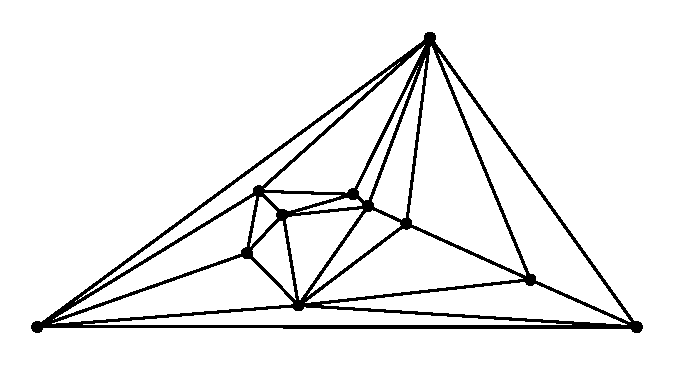
\includegraphics[width=\textwidth]{pics/text_1_int/pic_delaunay.pdf}
\caption{Splitting a face using Delaunay triangulation.}\label{fig:pic_delaunay}
\end{figure}

\begin{figure}[h]
\centering
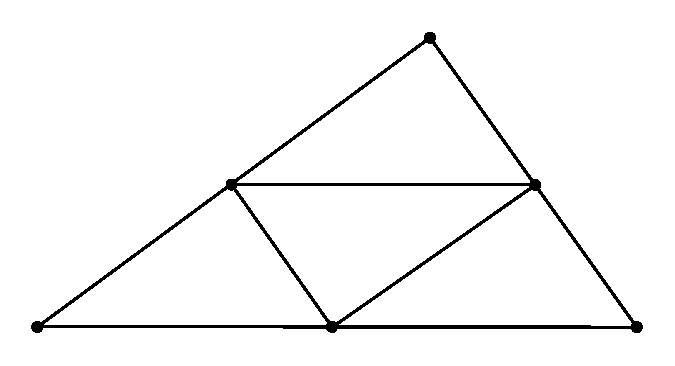
\includegraphics[width=\textwidth]{pics/text_1_int/pic_delaunay_2.pdf}
\caption{Breaking up a face into smaller ones.}\label{fig:pic_delaunay_2}
\end{figure}

\begin{figure}[h]
\centering
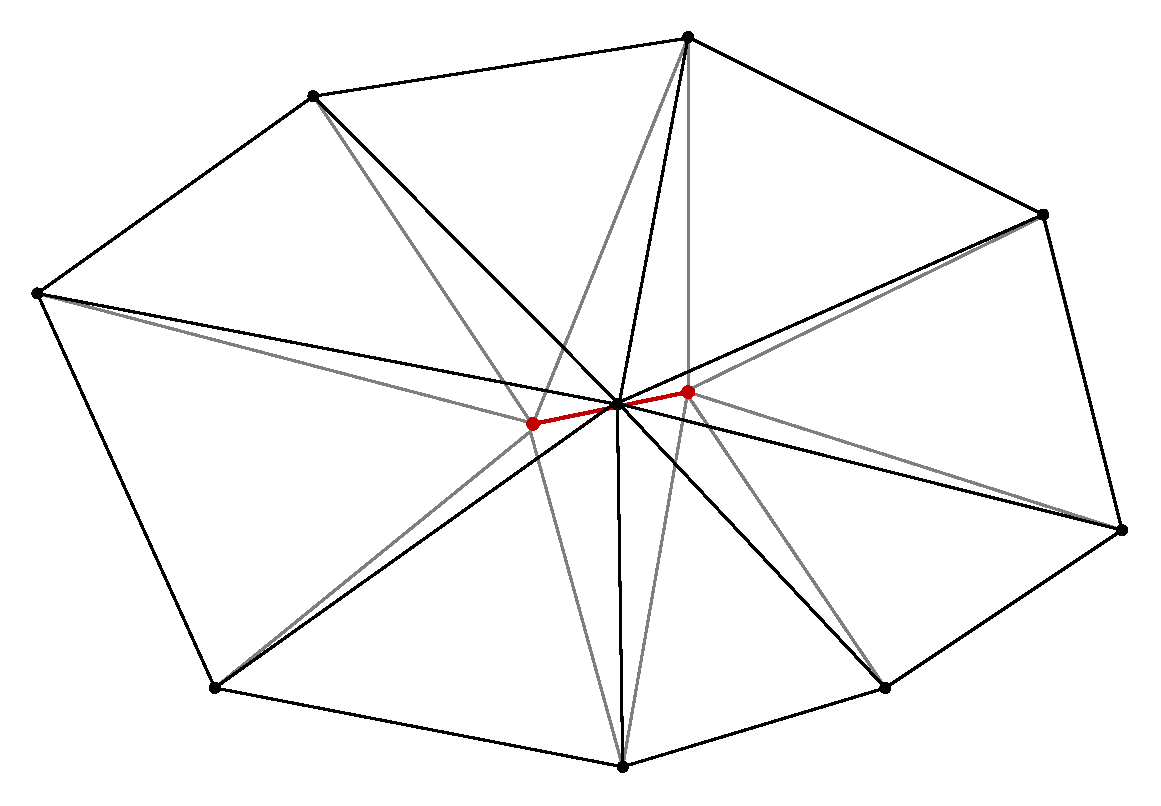
\includegraphics[width=\textwidth]{pics/text_1_int/pic_reduce_edge.pdf}
\caption{Edge reducing.}\label{fig:pic_reduce_edge}
\end{figure}

The first operation that we need is to split the face into smaller ones.
In all cases, we will split the faces using Delaunay triangulation, assuming that we know a set of points inside the face and we have to split the face using them (Fig.~\ref{fig:pic_delaunay}) \cite{Rivara}.
It is worth noting that face partitioning can be performed while preserving the local curvature of the mesh, as shown in \cite{Rakotoarivelo}, but for simplicity, we will partition only in the face plane.
If the split point is located not inside the face, but on its edge, then the second incident face of this edge will also have to be split (only meshes are considered whose edges have exactly two incident faces, as indicated in (\ref{eq_arch}).
Sometimes, to reduce the size, it is simply needed to split the face into smaller ones without setting split points.
In this case, it is necessary to monitor the quality of the resulting faces.
To determine the shape quality of a triangular face with nodes
$\vec{A}$, $\vec{B}$, $\vec{C}$, we can use a simple quality
criterion
\begin{equation*}
Q(f) = \frac{4\sqrt{3} S_{ABC}}{|\vec{AB}|^2 + |\vec{BC}|^2 +
|\vec{AC}|^2},
\end{equation*}
where $Q(f) = 1$ corresponds to the ideal case of an equilateral
face, and $Q(f) = 0$ is the worst case for faces with zero area
\cite{Borouchaki}.
To split a face into smaller ones while maintaining their quality, simply perform a split in the middle of all its sides (Fig.~\ref{fig:pic_delaunay_2}).

The second operation, which is necessary for mesh adaptation, is related to coarsening.
Quite often, when performing triangulation over a set of given points, faces with a low quality indicator may appear (they may have either too sharp corners or a corner close to $2 \pi$).
If the face contains an angle close to $2 \pi$, then splitting along the largest side will help to get rid of it (in this case, the base of the height lowered from the opposite node should be chosen as the splitting point).
If the triangle contains only close to acute angles, then it has a side that is too short, which can be removed.
When an edge $AB$ is removed, both faces incident to it are removed, nodes $A$ and $B$ are connected into a single node $A'$, and all edges from the set $\mathscr{E}(A) \cup \mathscr{E} (B)$ are redirected to node $A'$, taking into account the removal of doubles (Fig.~\ref{fig:pic_reduce_edge}).
This operation will be called edge reducing \cite{Panchal}.
By applying the reducing of the shortest edges in the  computational
mesh, we can achieve an arbitrary degree of coarsening.

%---------------------------------------------------------------------------------------------------

\subsubsection{Self-intersections elimination}

The main problem that can potentially be encountered in the evolution of the computational mesh is the occurrence of self-intersections.
Self-intersection is a critical mesh defect, which makes it impossible to perform further calculations on ice formation modeling, so self-intersections must be removed.
First, it is necessary to determine what ratio of two mesh faces can be interpreted as self-intersection.
Of course, the mere presence of common points in two faces cannot serve as a criterion for self-intersection, since each face has adjacent faces (that is, two faces can have both a common vertex and a common edge).
Since only faces that have common incident objects  (a common
incident vertex or a common incident edge) can be adjacent, and all
incidence relations are written in the computational mesh, it is not
difficult to separate the intersection of faces by a common incident
object from self-intersection.

\subsubsection{Search for pairs of intersecting triangles}

In any case, to identify all facts of mesh self-intersection, it is required to analyze all pairs of faces and check the intersection of faces in the pair (that is, check the intersection of each face with each).
Since direct enumeration of all faces pairs has quadratic complexity in terms of the number of faces in the mesh, so direct approach for large meshes is impossible.
In this case, it is advisable to search for pairs of intersecting faces using the representation of a set of faces in the form of a special tree structure associated with boxing of geometric objects by rectangular parallelepipeds in space.
First, let's define the concept of a container for an  arbitrary set
of points $M$ in space (we will denote it by $[M]$): $[M]$ is a
rectangular parallelepiped that is the Cartesian product of three
segments
\begin{equation*}
[M] = \left[\min_{P \in M}{P_x}, \max_{P \in M}{P_x}\right]
      \times \left[\min_{P \in M}{P_y}, \max_{P \in M}{P_y}\right]
      \times \left[\min_{P \in M}{P_z}, \max_{P \in M}{P_z}\right].
\end{equation*}

The container can be considered for an arbitrary set of points.
We will use it for a face of the computational mesh, as well as for a set of faces.
Since any triangle is a convex figure, then $[ABC] = [\{A, B, C\}]$, that is, to construct a container for a triangle, it is enough to consider only its vertices.
When searching for pairs of intersecting faces, we will use the following fact: if two triangles intersect, then their containers also intersect: $ABC \cap A'B'C' \ne \emptyset \Rightarrow [ABC] \cap [A'B'C'] \ne\emptyset$.
This means that if the containers of two triangles do not
intersect, then the triangles themselves do not intersect: $[ABC]
\cap [A'B'C'] = \emptyset \Rightarrow ABC \cap A'B'C' = \emptyset$.
Unlike the analysis of a pair of triangles for intersection,
checking for  the intersection of two rectangular boxes with sides
parallel to the coordinate axes is not a problem.
That is, at the first stage, we will look for such pairs of faces
whose  containers intersect (we will call them potentially
intersecting faces).

\begin{figure}[h]
\centering
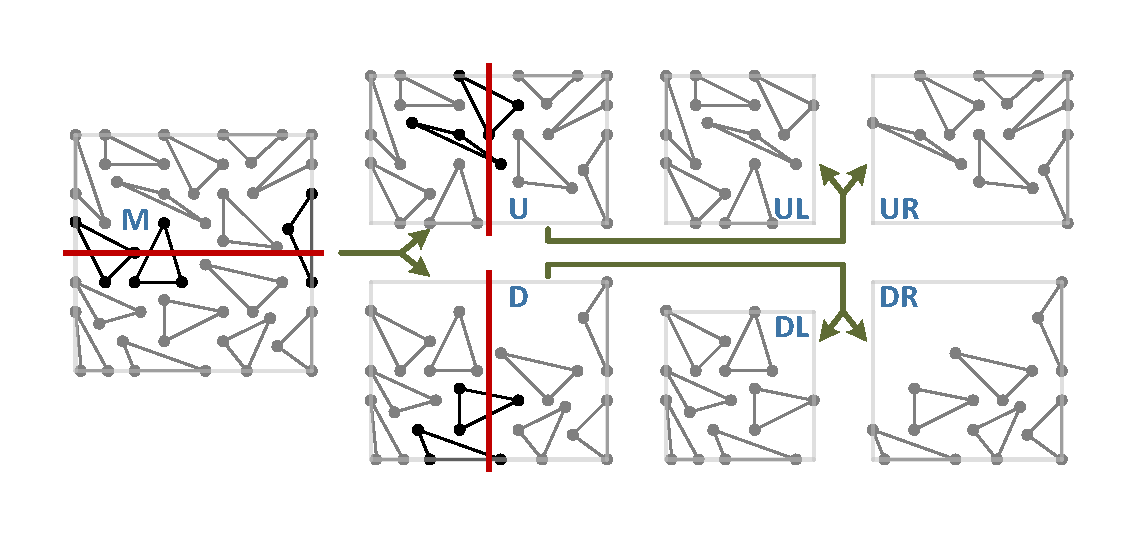
\includegraphics[width=0.8\textwidth]{pics/text_1_int/pic_box.pdf}
\captionstyle{center}\caption{Scheme for building a container tree.}\label{fig:pic_box}
\end{figure}

To search for potentially intersecting faces, we build a tree of
containers  for all mesh faces.
The root of this tree will be the container of all faces of the
computational  mesh.
Consider the procedure for dividing a container into two smaller
containers  using the two-dimensional case illustrated in
Fig.~\ref{fig:pic_box} as an example.
We want to divide the container of some set of triangles ($M$) along
a  horizontal straight line into two sets: upper set ($U$ -- up) and
lower set ($D$ -- down).
Then, all triangles that lie above the line or intersect it will
fall into the upper set.
Similarly, all triangles that lie below the line or intersect it will fall into the lower set.
After selecting the upper and lower sets of triangles, for each of them their own containers are built, which become child containers of the original one.
After that, the resulting containers can be divided further using an arbitrary splitting direction ($X$, $Y$, $Z$).
In particular, Fig.~\ref{fig:pic_box} demonstrates the splitting of the original container according to the scheme $[M] \rightarrow \{[U], [D]\} \rightarrow \{\{[UL], [UR]\}, \{[DL], [DR]\}\}$.
It should be noted that in one operation, a container can be split into an arbitrary number of child containers in a similar way.
As the direction of splitting the container, it is advisable to choose the most extended one (along which the length of the container has the greatest value).

The constructed container tree makes it possible to significantly reduce the number of tested potential intersections of triangles \cite{Jung}, since if $[M] \cap [M'] = \emptyset$, $[T]$ is a child container for $[M]$ , and $[T']$ is a child container for $[M']$, then $[T] \cap [T'] = \emptyset$.

After all pairs of potentially intersecting triangles have been found, it is necessary to check whether they actually intersect.
Since a triangle is a convex figure, the intersection of two triangles is also a convex figure (it can be any flat figure with 1 to 6 vertices).
The vertices of the intersection of two triangles are the points of intersection of the sides of one triangle with another triangle and vice versa.
Thus, the problem of finding the intersection of two triangles is reduced to finding the intersection points of a triangle and a segment.
This problem can be solved by representing triangle $ABC$ as a locus of points $\vec{P} = \vec{A} + \beta \vec{AB} + \gamma \vec{AC}$, $\beta \ge 0$, $\gamma \ge 0$, $\beta + \gamma \le 1$, representations of the segment $QR$ as the locus of points $\vec{P} = \vec{Q} + \phi \vec{QR}$, $0 \le \phi \le 1$ and finding a solution to the system of equations $\vec{A} + \beta \vec{AB} + \gamma \vec{AC} = \vec{Q} + \phi \vec{QR}$ with respect to the unknowns $\beta$, $\gamma$, $\phi$ subject to constraints \cite{Freylekhman}.

\subsubsection{Fixing intersecting triangles}

After all pairs of intersecting faces and areas of their intersections are found, it is necessary to determine a strategy for their elimination.
All faces of the computational mesh can be divided into three categories.
The first category is faces that do not intersect with any other faces, and which should become part of the final surface (we will assume that at any time we have the opportunity to specify an arbitrary number of such faces).
We will call such faces static.
The second category is faces that do not intersect with any other faces, but that should not become part of the final surface (faces of internal self-intersection loops of the surface that must be removed).
We will call such faces hidden.
The third category is faces that intersect with some other faces.
Such faces will be called intersection faces.

\begin{figure}[h]
\centering
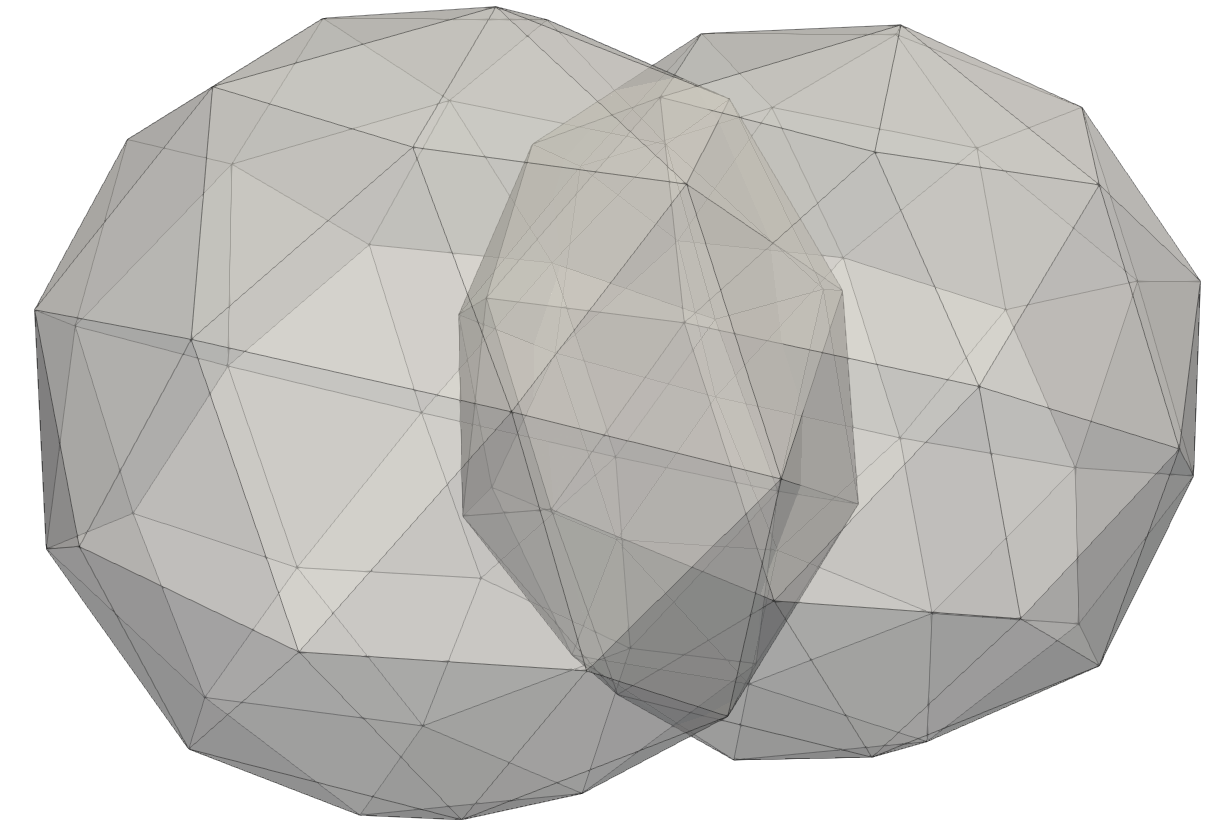
\includegraphics[width=\textwidth]{pics/text_1_int/pic_zip_01.png}
\caption{Intersection of computational meshes for two spheres.}\label{fig:pic_zip_01}
\end{figure}

\begin{figure}[h]
\centering
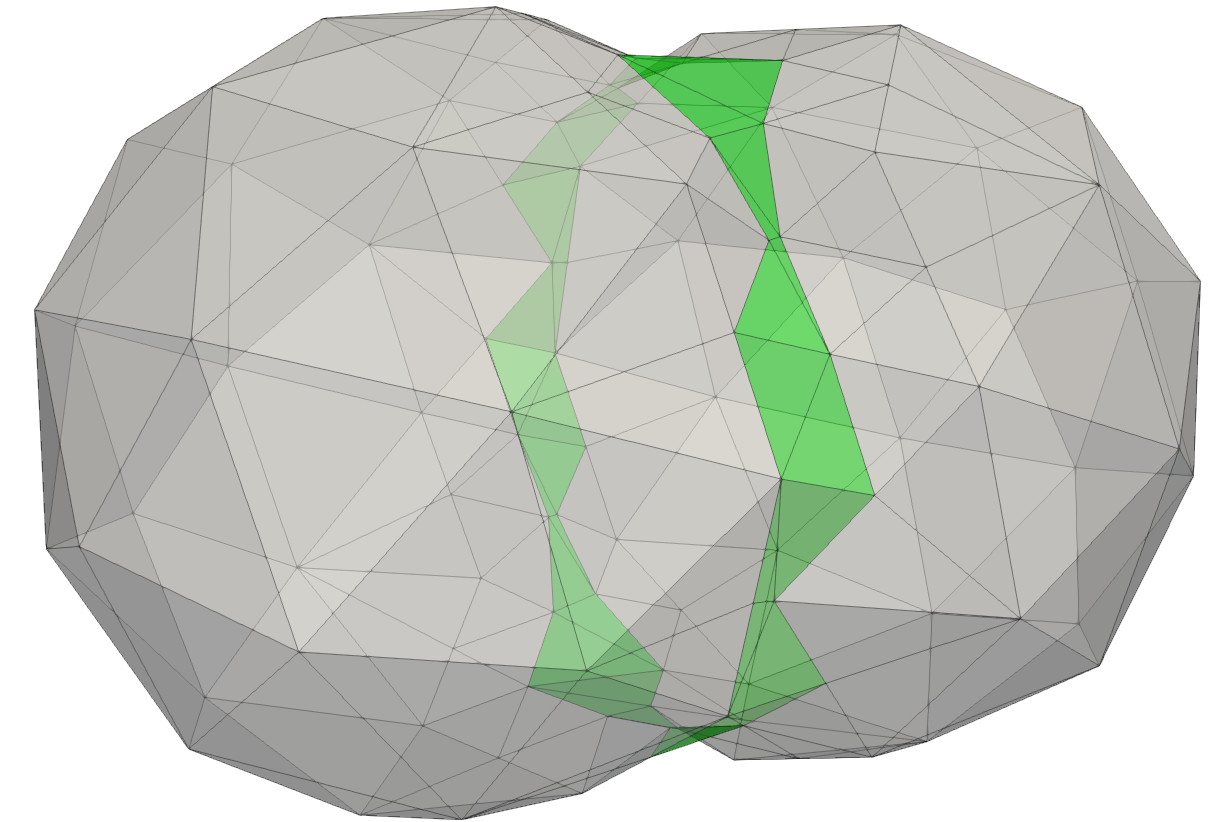
\includegraphics[width=\textwidth]{pics/text_1_int/pic_zip_09.png}
\caption{Rough removal of intersection faces.}\label{fig:pic_zip_09}
\end{figure}

\begin{figure}[h]
\centering
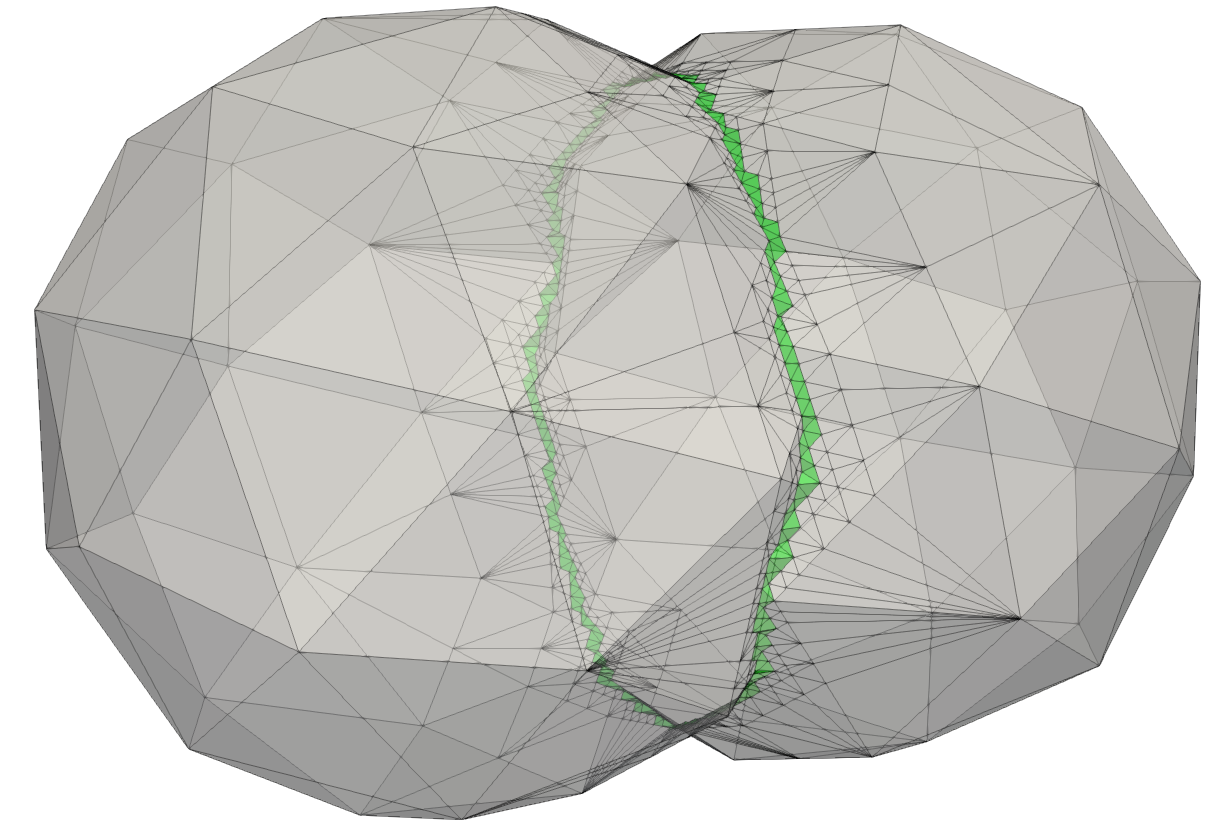
\includegraphics[width=\textwidth]{pics/text_1_int/pic_zip_15.png}
\caption{Removing intersection faces after splitting.}\label{fig:pic_zip_15}
\end{figure}

One approach to eliminating mesh self-intersections is to simply remove all intersection faces.
After performing this operation, the mesh is divided into areas of static and hidden faces.
In this case, the hidden faces are unreachable from the static areas when the faces of the computational mesh are bypassed (if only the faces adjacent along the edge are considered neighbors during the bypass).
After the hidden faces are removed from the mesh, the computational mesh consists only of static faces, but some new faces must be added to restore the integrity of the mesh \cite{Charton}.
This approach to eliminating mesh self-intersections can be used for relatively simple surfaces, but in general it does not guarantee a correct result.
As an illustration of such a way to eliminate intersections,
Figs.~\ref{fig:pic_zip_01} and~\ref{fig:pic_zip_09} shows an example
of work to eliminate intersections of the computational meshes of
two spheres (new faces that appear when the mesh is restored are
marked in green).
In Fig.~\ref{fig:pic_zip_09} we can note the rather low quality of the resulting mesh.
It is possible to improve the quality by splitting the intersection faces.
That is, after searching for all intersection faces, they must be split into smaller ones (as shown in Fig.~\ref{fig:pic_delaunay_2}), then repeat the procedure for deleting intersection faces and hidden faces and finally restore the mesh.
The process of splitting the intersection faces can be repeated many times, while the quality of the resulting mesh will increase, as shown in Fig.~\ref{fig:pic_zip_15}.

With another approach to eliminate self-intersections, no faces are removed from the mesh, but are split into smaller ones at all intersection points \cite{Skvorkovska}.
As an example, Fig.~\ref{fig:pic_before_cut} shows two triangles that intersect along a segment (two points of intersection).
After splitting, we get the construction shown in Fig.~\ref{fig:pic_after_cut}.
In the general case, there can be an arbitrarily large number of points at which it is necessary to split a face, and splitting should be performed by triangulating over these points, and some edges of the triangulation should be predefined.

\begin{figure}[h]
\centering
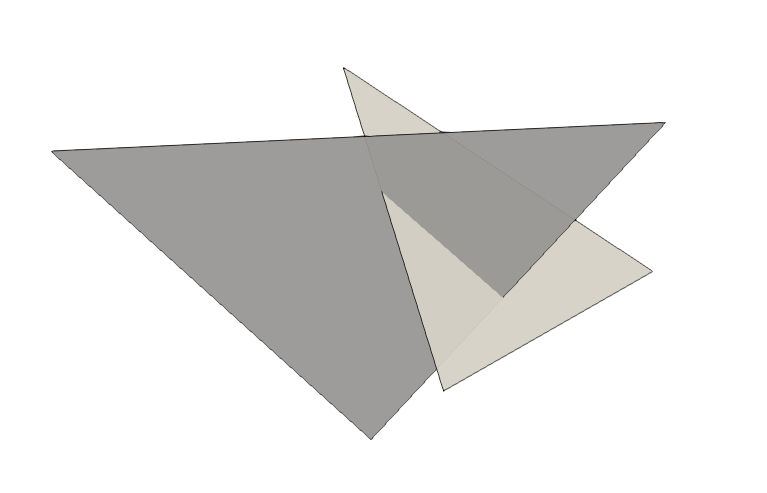
\includegraphics[width=\textwidth]{pics/text_1_int/pic_before_cut.png}
\end{figure}

\begin{figure}[h]
\centering
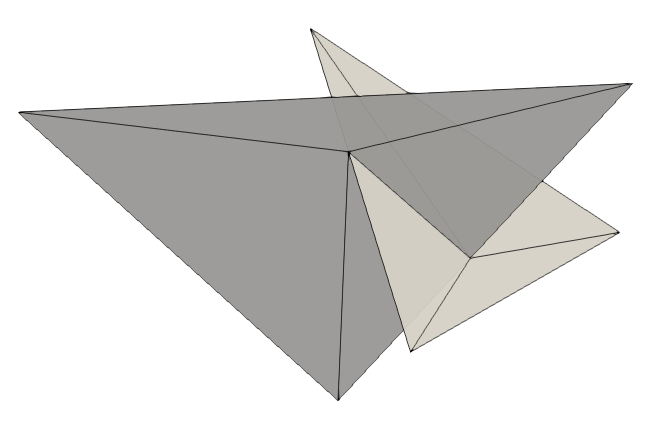
\includegraphics[width=\textwidth]{pics/text_1_int/pic_after_cut.png}
\caption{Faces after splitting by intersection points.}\label{fig:pic_after_cut}
\end{figure}

After splitting the faces by intersection points, only the following types of relations can remain between the faces of the mesh: two faces do not have common points, two faces have one common vertex, two faces have one common edge.
In this case, new edges that have more than two incident faces appear in our mesh.
If we impose two additional conditions on the original mesh, which can be achieved using local mesh transformations, then we can achieve a fairly simple mesh structure (we will call such meshes simple).
The first condition is the absence of matching vertices in the mesh.
The second condition is that no mesh node is located in any other face.
If these two additional conditions are satisfied, we can state that if an edge has more than two incident faces, then this number is exactly 4, and these 4 incident faces are pairwise in the same plane.

\begin{figure}[h]
\centering
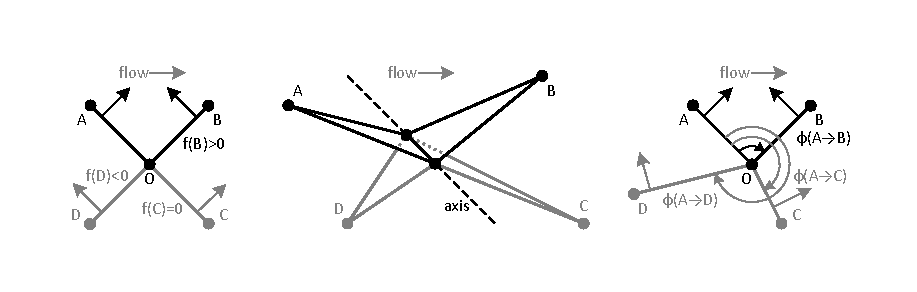
\includegraphics[width=0.85\textwidth]{pics/text_1_int/pic_walk_1.pdf}
\captionstyle{center}\caption{Scheme for bypassing the resulting surface.}\label{fig:pic_walk}
\end{figure}

To obtain the resulting surface, it is necessary to get rid of extra faces so that each edge again has exactly 2 incident faces.
To do this, it is necessary to traverse the mesh, starting from any static face, considering two faces adjacent that have a common incident edge (the faces marked during the traversal will be included into the resulting mesh).
When moving from a certain face through an edge that has more than two incident faces, the question arises of choosing a face that should enter the resulting mesh (while all other faces should be deleted).

Consider the procedure for selecting the next mesh walk face for edges with more than two incident faces (Fig.~\ref{fig:pic_walk}, center).
In this figure, the direction of traversal is indicated from left to right, after the face incident with the vertex $A$, the face incident with the vertex $B$ should enter the resulting mesh.
Consider this procedure for simple meshes, as well as for meshes in general.
For simplicity, we will consider the problem in projection onto a plane orthogonal to the edge.

\begin{figure}[h]
  \centering
  \begin{minipage}[h]{0.4\textwidth}
    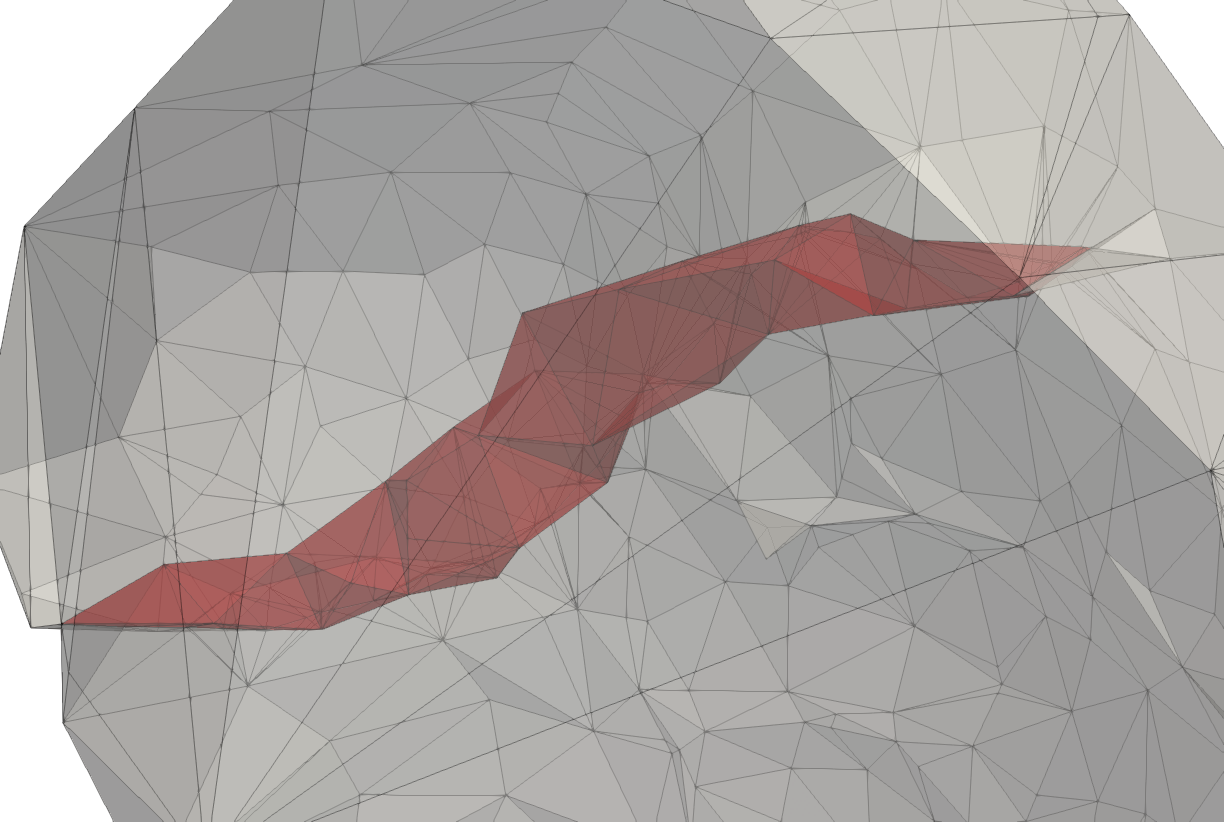
\includegraphics[width=\textwidth]{pics/text_1_int/pic_self_intersection_on.png}
    \caption{The surface before removing the self-intersection.}\label{fig:pic_self_intersection_on}
  \end{minipage}
  \begin{minipage}[h]{0.4\textwidth}
    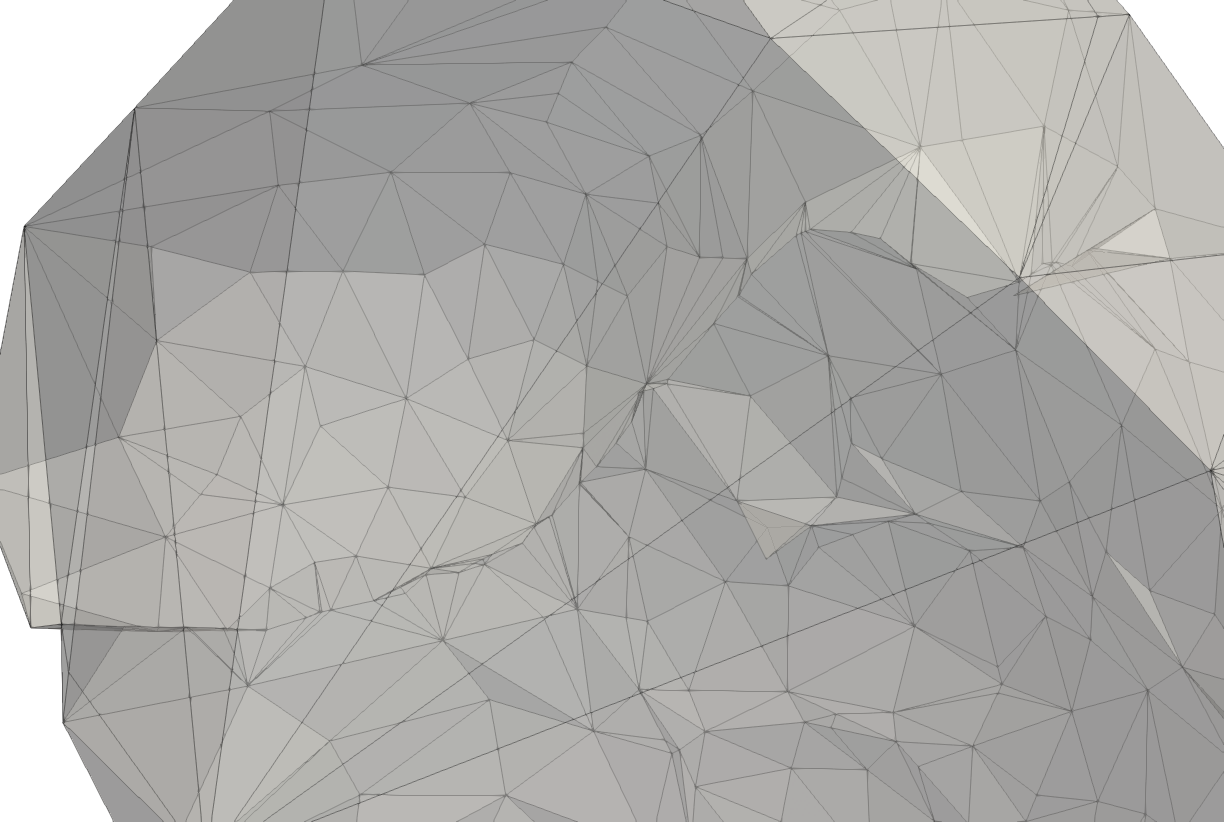
\includegraphics[width=\textwidth]{pics/text_1_int/pic_self_intersection_off.png}
    \caption{The surface after removing the self-intersection.}\label{fig:pic_self_intersection_off}
  \end{minipage}
\end{figure}

\begin{figure}[h]
  \centering
  \begin{minipage}[h]{0.4\textwidth}
    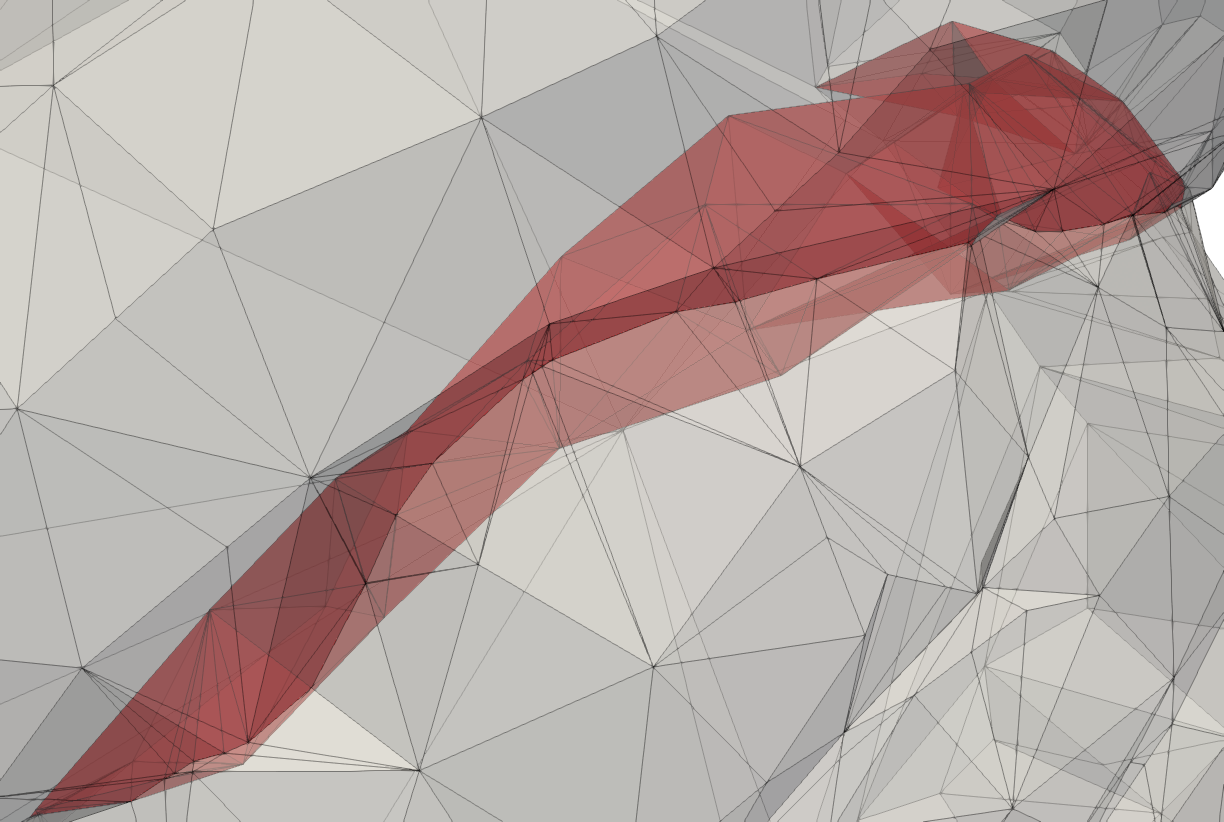
\includegraphics[width=\textwidth]{pics/text_1_int/pic_self_intersection_on_2.png}
    \caption{The surface before removing the self-intersection.}\label{fig:pic_self_intersection_on_2}
  \end{minipage}
  \begin{minipage}[h]{0.4\textwidth}
    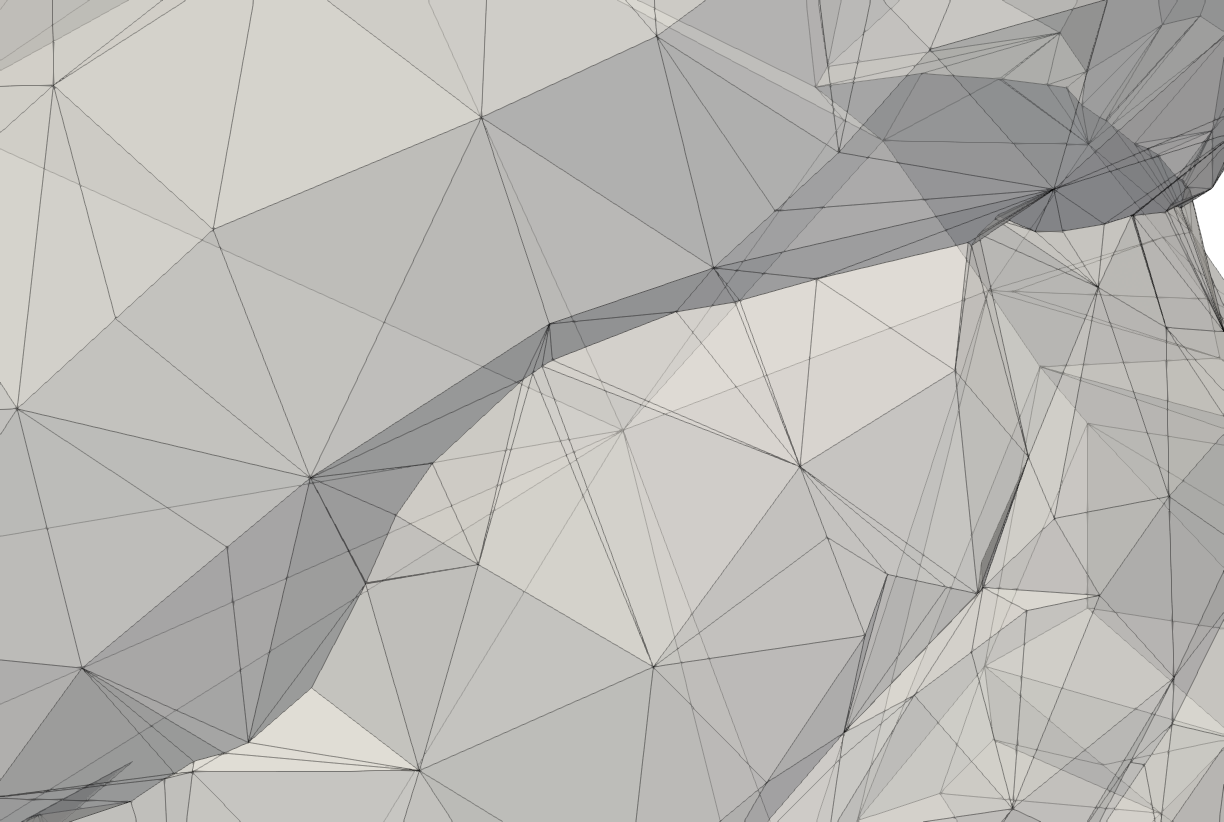
\includegraphics[width=\textwidth]{pics/text_1_int/pic_self_intersection_off_2.png}
    \caption{The surface after removing the self-intersection.}\label{fig:pic_self_intersection_off_2}
  \end{minipage}
\end{figure}

To begin with, we will assume that the case of a simple mesh takes place (Fig.~\ref{fig:pic_walk}, left).
Let it be already known that the face incident to the vertex $A$ is labeled and its outward normal denoted by $\vec{n}_A$.
Of the remaining three faces (incidental to the vertices $B$, $C$, $D$, respectively), it is necessary to choose only one to continue traversing the mesh, and delete the rest.
Since we have a simple mesh, then $\angle AOC = \angle BOD = 2 \pi$, which means $(\vec{n}_A, \vec{OB}) > 0$, $(\vec{n} _A, \vec{OC}) = 0$, $(\vec{n}_A, \vec{OD}) < 0$.
Thus, from all faces, it is necessary to choose the one for which the value of $(\vec{n}_A, \vec{OP})$ is maximum.

Now consider the computational mesh in general case.
In this case, the number of faces incident to the considered edge can be arbitrary, more than two, and nothing can be said about the value of the function $(\vec{n}_A, \vec{OP})$.
To select the next face to bypass the mesh, we will rotate the current face around the considered edge in the direction of $\vec{n}_A$ until it coincides with the first face (Fig.~\ref{fig:pic_walk}, on the right).
The first face must be selected as the next one to continue the mesh traverse.
If we denote by $\phi(A \rightarrow P)$ the angle of rotation of the original face in the direction $\vec{n}_A$ to the face incident with the vertex $P$, then the face for which $\phi(A \rightarrow B)$ will be minimal should be selected as the next one for traverse.

Combining both considered cases together, we obtain  a criterion for
choosing the next face to bypass: a face must be chosen for which
the value of the function $f(P)$ is maximum, where
\begin{equation*}
f(P) =
\begin{cases}
(\vec{n}_A, \vec{OP}), \text{for simple meshes}, \\
-\phi(A \rightarrow P), \text{for general case meshes}
\end{cases}
\end{equation*}
After completion of the computational mesh bypass, all marked faces are considered to be faces of the target surface, and all other faces must be deleted.
Figures
\ref{fig:pic_self_intersection_on}--\ref{fig:pic_self_intersection_off_2}
illustrate examples of eliminating mesh self-intersections in the
form of hidden loops.
After removing the hidden faces, the target computational mesh again becomes correct, satisfies the relations (\ref{eq_arch}) and can be used for further ice formation modeling.
